% 图 77.2 —— 由 `checks/emit_hand.py` 自动拼出（probe 精测 + prims2 图元分解）
%%
% ⚠ 这是**稿子不是成品**：跑 `checks/checkhand.py 77.2` 看指标 + 看叠合图。
%%
%% ⚠ 待核：
%   · 本图 probe 报出阴影族 3 个 —— **本脚本不生成阴影**（要照原书手写）；prims2 的 strokes 里可能含阴影线，核对时留意别画重
%   · 可疑字形 1 项（空心圈 ⊙ 常被认成字母 o）—— 见文件末
%%
\documentclass[12pt]{standalone}
\usepackage{fontspec}
\setsansfont{Arial}
\newfontfamily\mfallback{DejaVu Sans}
\usepackage{tikz}
\begin{document}
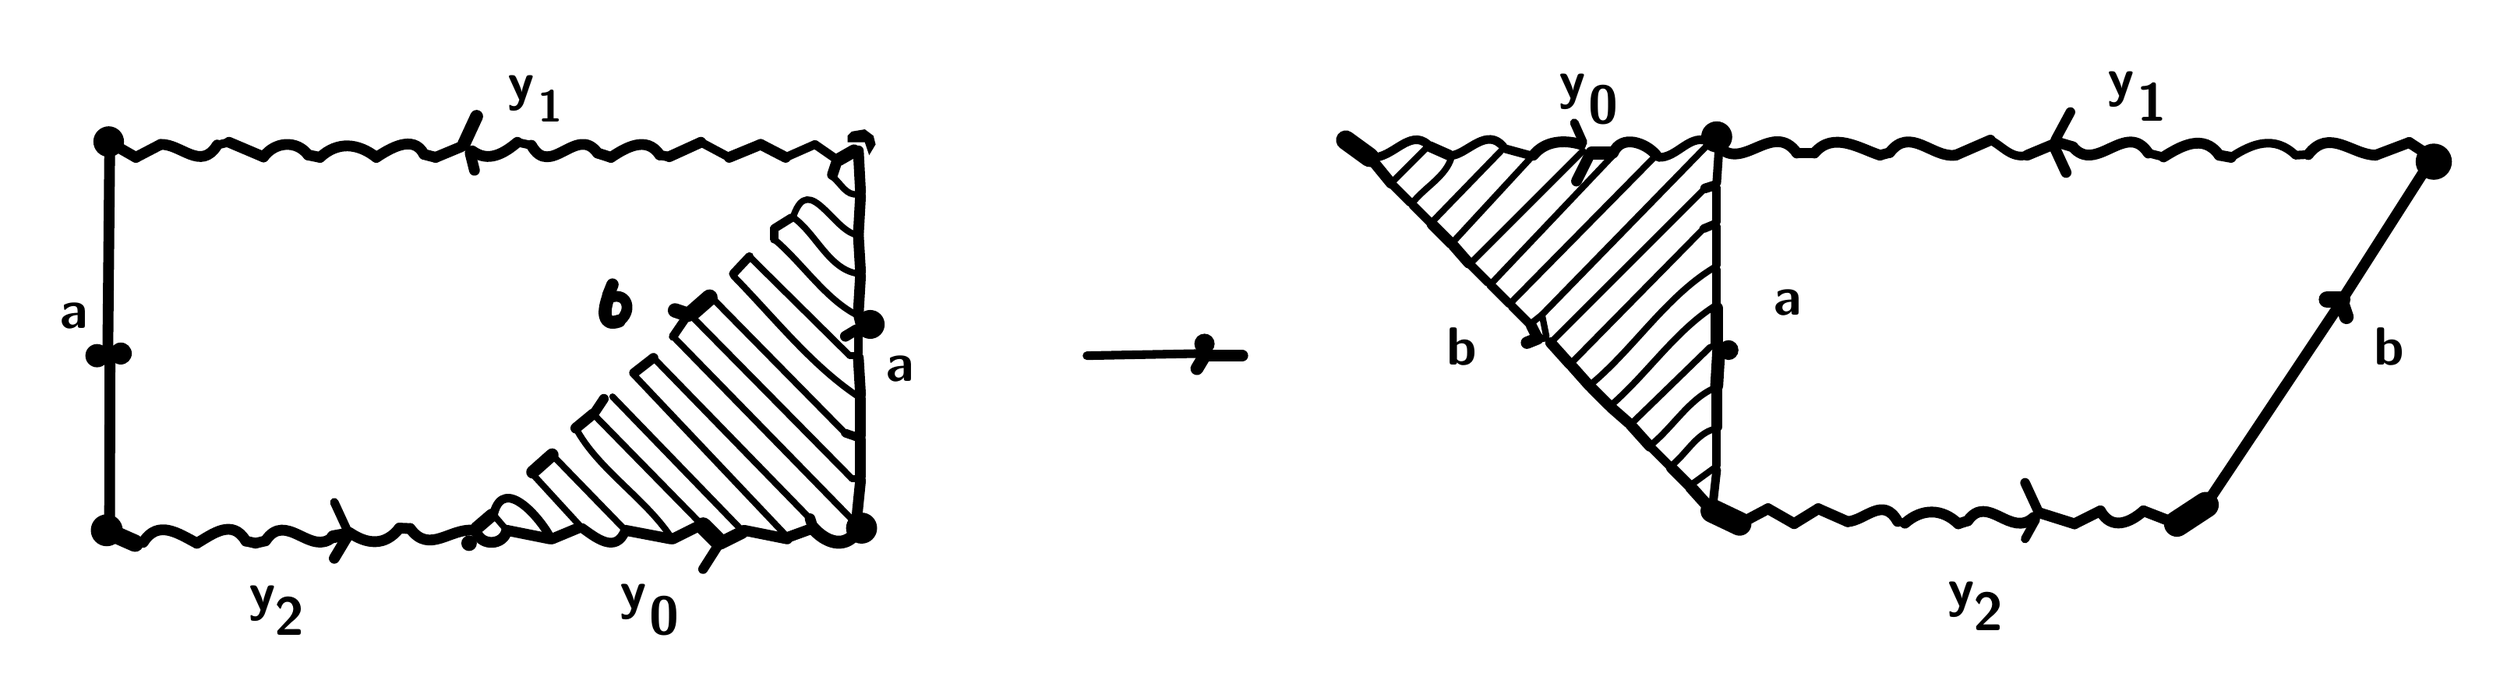
\begin{tikzpicture}[x=1pt, y=-1pt, line width=3.0pt, line cap=round, line join=round]

  %% ════ 填充区（prims2 的 fills）════
  \fill (385.0,51.0) -- (383.0,53.0) -- (383.0,56.0) -- (391.0,56.0) -- (393.0,62.0) -- (396.0,57.0) -- (395.0,53.0) -- (391.0,50.0) -- cycle;

  %% ════ 直线段（prims2 的 strokes）════
  \draw[line width=3.0pt] (219.0,229.0) -- (225.0,236.0);
  \draw[line width=5.5pt] (549.0,155.0) -- (566.0,155.0);
  \draw[line width=7.7pt] (1076.0,129.0) -- (1069.0,129.0);
  \draw[line width=5.0pt] (1076.0,129.0) -- (1118.0,63.2);
  \draw[line width=5.0pt] (1118.0,63.2) -- (1107.1,56.1);
  \draw[line width=5.0pt] (1107.1,56.1) -- (1091.5,62.0);
  \draw[line width=4.0pt] (1060.3,61.7) -- (1054.4,62.0);
  \draw[line width=5.0pt] (1024.5,63.0) -- (1019.0,62.0);
  \draw[line width=4.0pt] (993.2,62.8) -- (986.1,61.0);
  \draw[line width=5.0pt] (951.1,58.1) -- (944.0,56.0);
  \draw[line width=8.0pt] (323.0,241.0) -- (316.0,234.0);
  \draw[line width=3.0pt] (706.0,147.0) -- (703.0,147.0);
  \draw[line width=4.0pt] (934.0,231.0) -- (929.0,240.0);
  \draw[line width=4.0pt] (688.0,59.0) -- (699.0,62.0);
  \draw[line width=5.0pt] (151.0,239.0) -- (145.0,249.0);
  \draw[line width=5.0pt] (654.0,94.0) -- (663.0,103.0);
  \draw[line width=4.5pt] (785.0,76.0) -- (780.6,77.4);
  \draw[line width=3.0pt] (780.6,77.4) -- (710.0,148.0);
  \draw[line width=3.0pt] (274.0,174.0) -- (334.0,236.0);
  \draw[line width=6.0pt] (246.0,201.0) -- (237.0,209.0);
  \draw[line width=3.0pt] (246.0,201.0) -- (280.0,236.0);
  \draw[line width=5.5pt] (774.0,216.0) -- (783.0,226.0);
  \draw[line width=5.0pt] (246.0,240.0) -- (258.0,235.0);
  \draw[line width=4.0pt] (756.0,198.0) -- (764.0,206.0);
  \draw[line width=4.3pt] (389.0,141.0) -- (388.0,137.0);
  \draw[line width=4.0pt] (672.0,113.0) -- (680.0,121.0);
  \draw[line width=6.0pt] (218.0,229.0) -- (211.0,235.0);
  \draw[line width=5.0pt] (948.0,70.0) -- (942.0,57.0);
  \draw[line width=6.0pt] (379.0,64.0) -- (386.0,60.0);
  \draw[line width=3.0pt] (783.0,151.0) -- (747.0,186.0);
  \draw[line width=6.0pt] (728.0,61.0) -- (737.0,61.0);
  \draw[line width=5.0pt] (626.0,64.0) -- (635.0,75.0);
  \draw[line width=4.0pt] (547.0,154.0) -- (494.0,155.0);
  \draw[line width=6.0pt] (334.0,237.0) -- (324.0,242.0);
  \draw[line width=4.0pt] (636.0,76.0) -- (644.0,84.0);
  \draw[line width=3.0pt] (738.0,62.0) -- (682.0,121.0);
  \draw[line width=5.0pt] (721.0,74.0) -- (727.0,62.0);
  \draw[line width=5.0pt] (225.0,236.0) -- (245.0,240.0);
  \draw[line width=5.0pt] (1075.0,131.0) -- (1012.8,224.2);
  \draw[line width=12.0pt] (1012.8,224.2) -- (999.4,233.0);
  \draw[line width=5.0pt] (999.4,233.0) -- (983.9,227.0);
  \draw[line width=5.0pt] (963.9,227.0) -- (951.9,233.0);
  \draw[line width=5.0pt] (951.9,233.0) -- (936.0,228.0);
  \draw[line width=5.0pt] (719.0,160.0) -- (727.0,169.0);
  \draw[line width=5.0pt] (356.0,239.0) -- (367.0,235.0);
  \draw[line width=5.9pt] (150.0,238.0) -- (144.4,239.0);
  \draw[line width=4.9pt] (113.1,240.9) -- (108.5,242.0);
  \draw[line width=4.9pt] (108.5,242.0) -- (104.0,241.0);
  \draw[line width=3.9pt] (56.4,241.6) -- (52.6,242.0);
  \draw[line width=8.0pt] (52.6,242.0) -- (40.8,236.8);
  \draw[line width=5.0pt] (40.8,236.8) -- (41.0,154.0);
  \draw[line width=5.0pt] (210.0,69.0) -- (208.0,61.0);
  \draw[line width=5.0pt] (389.0,116.0) -- (388.0,99.0);
  \draw[line width=5.3pt] (783.0,56.0) -- (787.0,58.0);
  \draw[line width=3.0pt] (783.0,56.0) -- (705.0,136.0);
  \draw[line width=6.7pt] (303.0,134.0) -- (309.0,136.0);
  \draw[line width=4.0pt] (378.0,64.0) -- (367.9,57.0);
  \draw[line width=4.0pt] (367.9,57.0) -- (354.3,63.0);
  \draw[line width=5.0pt] (354.3,63.0) -- (342.7,57.0);
  \draw[line width=5.0pt] (342.7,57.0) -- (328.1,63.0);
  \draw[line width=4.0pt] (328.1,63.0) -- (315.0,56.0);
  \draw[line width=5.0pt] (315.0,56.0) -- (300.3,62.7);
  \draw[line width=4.5pt] (300.3,62.7) -- (295.9,61.9);
  \draw[line width=5.0pt] (273.3,63.0) -- (267.1,61.0);
  \draw[line width=4.0pt] (236.4,57.4) -- (229.9,56.0);
  \draw[line width=5.0pt] (737.0,179.0) -- (745.0,186.0);
  \draw[line width=5.7pt] (272.0,127.0) -- (274.0,122.0);
  \draw[line width=5.0pt] (388.0,135.0) -- (389.0,118.0);
  \draw[line width=4.5pt] (266.0,181.0) -- (270.0,175.0);
  \draw[line width=6.0pt] (786.0,169.0) -- (787.0,152.0);
  \draw[line width=4.0pt] (786.0,131.0) -- (786.0,115.0);
  \draw[line width=4.9pt] (367.0,235.0) -- (365.6,230.6);
  \draw[line width=3.0pt] (365.6,230.6) -- (293.0,156.0);
  \draw[line width=4.5pt] (293.0,156.0) -- (284.0,163.0);
  \draw[line width=5.0pt] (736.0,178.0) -- (728.0,170.0);
  \draw[line width=3.0pt] (259.0,234.0) -- (237.0,210.0);
  \draw[line width=4.0pt] (388.0,154.0) -- (388.0,144.0);
  \draw[line width=5.0pt] (709.0,149.0) -- (718.0,159.0);
  \draw[line width=5.0pt] (302.0,240.0) -- (314.0,234.0);
  \draw[line width=4.0pt] (388.0,193.0) -- (381.9,190.9);
  \draw[line width=3.0pt] (381.9,190.9) -- (320.0,128.0);
  \draw[line width=3.0pt] (355.0,239.0) -- (284.0,164.0);
  \draw[line width=5.0pt] (786.0,188.0) -- (786.0,170.0);
  \draw[line width=4.0pt] (786.0,93.0) -- (786.0,77.0);
  \draw[line width=5.0pt] (387.0,143.0) -- (382.0,146.0);
  \draw[line width=6.0pt] (786.0,150.0) -- (786.0,133.0);
  \draw[line width=4.0pt] (151.0,236.0) -- (145.0,223.0);
  \draw[line width=3.0pt] (388.0,212.0) -- (385.0,212.0);
  \draw[line width=3.0pt] (385.0,212.0) -- (311.0,137.0);
  \draw[line width=5.0pt] (175.2,235.0) -- (180.2,235.2);
  \draw[line width=3.0pt] (691.0,130.0) -- (757.0,63.0);
  \draw[line width=5.0pt] (376.0,71.0) -- (378.0,65.0);
  \draw[line width=3.0pt] (785.0,207.0) -- (774.0,215.0);
  \draw[line width=5.0pt] (40.0,152.0) -- (40.9,56.1);
  \draw[line width=5.0pt] (40.9,56.1) -- (53.0,63.0);
  \draw[line width=5.0pt] (53.0,63.0) -- (64.5,57.0);
  \draw[line width=4.0pt] (90.7,57.3) -- (96.2,56.0);
  \draw[line width=5.0pt] (96.2,56.0) -- (112.2,62.8);
  \draw[line width=5.0pt] (132.9,61.9) -- (138.4,63.0);
  \draw[line width=5.0pt] (186.6,61.6) -- (192.0,63.0);
  \draw[line width=5.0pt] (192.0,63.0) -- (204.0,58.0);
  \draw[line width=5.0pt] (823.2,61.0) -- (831.3,61.0);
  \draw[line width=4.8pt] (861.7,62.0) -- (866.2,60.8);
  \draw[line width=5.0pt] (896.8,62.0) -- (912.9,55.0);
  \draw[line width=5.0pt] (930.0,62.0) -- (942.0,57.0);
  \draw[line width=5.0pt] (301.0,240.0) -- (280.0,236.0);
  \draw[line width=5.0pt] (700.0,141.0) -- (703.0,147.0);
  \draw[line width=4.5pt] (950.0,42.0) -- (943.0,55.0);
  \draw[line width=9.0pt] (614.0,55.0) -- (625.0,63.0);
  \draw[line width=4.5pt] (316.0,254.0) -- (323.0,243.0);
  \draw[line width=5.0pt] (664.0,104.0) -- (671.0,112.0);
  \draw[line width=4.0pt] (681.0,122.0) -- (690.0,131.0);
  \draw[line width=3.0pt] (387.0,233.0) -- (302.1,146.1);
  \draw[line width=4.0pt] (302.1,146.1) -- (309.0,136.0);
  \draw[line width=5.0pt] (387.0,233.0) -- (389.0,213.0);
  \draw[line width=4.0pt] (784.0,226.0) -- (786.0,208.0);
  \draw[line width=3.0pt] (724.0,60.0) -- (672.0,112.0);
  \draw[line width=6.0pt] (548.0,156.0) -- (545.0,161.0);
  \draw[line width=5.0pt] (662.0,62.0) -- (653.0,58.0);
  \draw[line width=3.0pt] (636.0,74.0) -- (651.0,59.0);
  \draw[line width=4.0pt] (645.0,85.0) -- (653.0,93.0);
  \draw[line width=3.0pt] (705.0,136.0) -- (700.0,140.0);
  \draw[line width=3.0pt] (705.0,136.0) -- (707.0,146.0);
  \draw[line width=5.0pt] (765.0,207.0) -- (773.0,215.0);
  \draw[line width=7.5pt] (319.0,128.0) -- (311.0,135.0);
  \draw[line width=4.5pt] (935.0,227.0) -- (929.0,214.0);
  \draw[line width=5.0pt] (746.0,187.0) -- (755.0,197.0);
  \draw[line width=3.0pt] (719.0,158.0) -- (779.9,96.1);
  \draw[line width=4.0pt] (779.9,96.1) -- (785.0,94.0);
  \draw[line width=4.0pt] (786.0,206.0) -- (786.0,190.0);
  \draw[line width=5.0pt] (389.0,194.0) -- (389.0,211.0);
  \draw[line width=4.0pt] (720.0,47.0) -- (724.0,56.0);
  \draw[line width=3.0pt] (686.0,60.0) -- (654.0,93.0);
  \draw[line width=5.0pt] (389.0,175.0) -- (389.0,192.0);
  \draw[line width=5.0pt] (389.0,79.0) -- (388.0,60.0);
  \draw[line width=3.0pt] (664.0,102.0) -- (700.0,63.0);
  \draw[line width=5.0pt] (335.0,236.0) -- (355.0,240.0);
  \draw[line width=4.0pt] (786.0,113.0) -- (786.0,95.0);
  \draw[line width=4.0pt] (786.0,75.0) -- (787.0,60.0);
  \draw[line width=11.0pt] (784.0,227.0) -- (796.6,233.0);
  \draw[line width=5.0pt] (796.6,233.0) -- (809.8,226.0);
  \draw[line width=5.0pt] (809.8,226.0) -- (821.9,232.9);
  \draw[line width=5.0pt] (821.9,232.9) -- (833.1,226.0);
  \draw[line width=5.0pt] (833.1,226.0) -- (846.7,232.0);
  \draw[line width=3.7pt] (869.9,231.9) -- (873.3,232.7);
  \draw[line width=4.9pt] (898.0,233.0) -- (902.4,231.6);
  \draw[line width=4.0pt] (349.0,101.0) -- (349.0,96.0);
  \draw[line width=4.0pt] (349.0,96.0) -- (357.0,91.0);
  \draw[line width=5.7pt] (698.0,149.0) -- (703.0,147.0);
  \draw[line width=6.7pt] (1076.0,131.0) -- (1078.0,137.0);
  \draw[line width=3.0pt] (387.0,155.0) -- (384.0,155.0);
  \draw[line width=3.0pt] (384.0,155.0) -- (337.5,109.0);
  \draw[line width=4.0pt] (337.5,109.0) -- (330.0,117.0);
  \draw[line width=3.0pt] (315.0,233.0) -- (266.0,183.0);
  \draw[line width=5.0pt] (389.0,173.0) -- (388.0,156.0);
  \draw[line width=6.0pt] (205.0,57.0) -- (211.0,44.0);
  \draw[line width=5.0pt] (257.0,188.6) -- (265.0,182.0);
  \draw[line width=4.0pt] (691.0,132.0) -- (699.0,140.0);
  \draw[line width=5.0pt] (389.0,81.0) -- (388.0,99.0);

  %% ════ 曲线（prims2 的 curves —— 三段式，坐标同为 (y,x)）════
  \draw[line width=3.0pt] (765.0,206.0) .. controls (771.8,200.7) and (776.6,191.1) .. (785.0,189.0);
  \draw[line width=5.0pt] (1091.5,62.0) .. controls (1080.5,61.8) and (1070.0,49.1) .. (1060.3,61.7);
  \draw[line width=4.0pt] (1054.4,62.0) .. controls (1044.7,52.7) and (1034.5,56.4) .. (1024.5,63.0);
  \draw[line width=5.0pt] (1019.0,62.0) .. controls (1011.7,51.6) and (1000.9,58.0) .. (993.2,62.8);
  \draw[line width=5.0pt] (986.1,61.0) .. controls (975.9,45.6) and (961.9,71.1) .. (951.1,58.1);
  \draw[line width=3.0pt] (785.0,114.0) .. controls (762.9,127.2) and (747.7,151.5) .. (728.0,168.0);
  \draw[line width=4.0pt] (245.0,239.0) .. controls (240.8,231.0) and (223.9,210.4) .. (219.0,228.0);
  \draw[line width=5.0pt] (225.0,236.0) .. controls (223.6,243.1) and (213.3,243.5) .. (211.0,237.0);
  \draw[line width=5.0pt] (983.9,227.0) .. controls (977.9,232.3) and (969.2,236.4) .. (963.9,227.0);
  \draw[line width=5.0pt] (144.4,239.0) .. controls (134.2,248.6) and (122.6,226.6) .. (113.1,240.9);
  \draw[line width=5.0pt] (104.0,241.0) .. controls (97.7,230.3) and (88.4,237.9) .. (81.3,242.0);
  \draw[line width=5.0pt] (81.3,242.0) .. controls (72.9,237.6) and (63.2,230.7) .. (56.4,241.6);
  \draw[line width=4.5pt] (260.0,235.0) .. controls (265.9,239.2) and (275.6,247.3) .. (280.0,236.0);
  \draw[line width=4.0pt] (783.0,56.0) .. controls (773.8,51.0) and (767.8,63.5) .. (759.0,63.0);
  \draw[line width=5.0pt] (295.9,61.9) .. controls (289.8,52.6) and (279.8,58.7) .. (273.3,63.0);
  \draw[line width=5.0pt] (267.1,61.0) .. controls (257.4,47.6) and (245.2,73.2) .. (236.4,57.4);
  \draw[line width=5.0pt] (229.9,56.0) .. controls (223.8,61.1) and (216.5,65.6) .. (209.0,60.0);
  \draw[line width=5.0pt] (701.0,62.0) .. controls (706.4,55.3) and (715.2,54.7) .. (723.0,57.0);
  \draw[line width=5.0pt] (273.0,128.0) .. controls (281.5,125.1) and (283.2,135.1) .. (277.1,138.9);
  \draw[line width=6.0pt] (277.1,138.9) .. controls (268.6,141.9) and (270.2,133.0) .. (272.0,128.0);
  \draw[line width=3.0pt] (358.0,90.0) .. controls (365.3,69.3) and (377.0,98.4) .. (388.0,99.0);
  \draw[line width=6.0pt] (367.0,235.0) .. controls (372.4,241.2) and (381.2,245.0) .. (387.0,237.0);
  \draw[line width=3.0pt] (330.0,118.0) .. controls (348.7,137.0) and (366.2,159.5) .. (388.0,174.0);
  \draw[line width=4.0pt] (664.0,62.0) .. controls (671.1,60.4) and (679.6,49.2) .. (687.0,58.0);
  \draw[line width=5.0pt] (152.0,237.0) .. controls (160.0,242.5) and (168.5,243.6) .. (175.2,235.0);
  \draw[line width=5.0pt] (180.2,235.2) .. controls (189.1,247.4) and (198.9,234.6) .. (210.0,236.0);
  \draw[line width=5.0pt] (64.5,57.0) .. controls (73.9,56.6) and (83.1,69.6) .. (90.7,57.3);
  \draw[line width=5.0pt] (112.2,62.8) .. controls (117.3,55.8) and (127.4,54.7) .. (132.9,61.9);
  \draw[line width=5.0pt] (138.4,63.0) .. controls (146.6,55.4) and (156.1,56.4) .. (164.5,63.0);
  \draw[line width=5.0pt] (164.5,63.0) .. controls (170.5,59.1) and (181.7,52.0) .. (186.6,61.6);
  \draw[line width=5.0pt] (788.0,59.0) .. controls (798.8,68.5) and (812.5,46.1) .. (823.2,61.0);
  \draw[line width=5.0pt] (831.3,61.0) .. controls (840.1,50.7) and (852.2,58.9) .. (861.7,62.0);
  \draw[line width=5.0pt] (866.2,60.8) .. controls (875.7,48.3) and (886.0,63.5) .. (896.8,62.0);
  \draw[line width=4.0pt] (912.9,55.0) .. controls (918.6,57.8) and (922.7,64.0) .. (930.0,62.0);
  \draw[line width=3.0pt] (756.0,196.0) .. controls (765.9,187.8) and (773.5,174.9) .. (785.0,170.0);
  \draw[line width=3.0pt] (645.0,84.0) .. controls (650.6,76.9) and (660.6,71.7) .. (663.0,63.0);
  \draw[line width=3.0pt] (376.0,72.0) .. controls (379.9,74.9) and (382.4,81.3) .. (388.0,80.0);
  \draw[line width=3.0pt] (358.0,91.0) .. controls (368.6,98.7) and (374.6,115.2) .. (388.0,117.0);
  \draw[line width=3.0pt] (785.0,132.0) .. controls (766.7,143.7) and (753.9,163.3) .. (737.0,178.0);
  \draw[line width=5.0pt] (846.7,232.0) .. controls (855.0,231.4) and (863.2,219.9) .. (869.9,231.9);
  \draw[line width=5.0pt] (873.3,232.7) .. controls (881.2,225.7) and (890.6,225.8) .. (898.0,233.0);
  \draw[line width=5.0pt] (902.4,231.6) .. controls (911.7,218.6) and (922.2,239.9) .. (933.0,230.0);
  \draw[line width=3.0pt] (387.0,136.0) .. controls (372.6,128.5) and (362.0,112.0) .. (349.0,101.0);
  \draw[line width=5.0pt] (738.0,61.0) .. controls (741.8,52.0) and (753.3,56.3) .. (758.0,62.0);
  \draw[line width=4.0pt] (626.0,63.0) .. controls (635.5,63.9) and (643.6,49.5) .. (652.0,57.0);
  \draw[line width=3.0pt] (301.0,239.0) .. controls (288.9,220.9) and (267.1,207.6) .. (257.0,188.6);

  %% ════ 实心点 ════
  \fill (786.0,53.5) circle (7.2);
  \fill (40.4,55.7) circle (7.1);
  \fill (1118.5,65.0) circle (8.4);
  \fill (393.5,140.5) circle (6.7);
  \fill (46.0,154.0) circle (5.1);
  \fill (548.5,149.5) circle (4.7);
  \fill (791.5,152.4) circle (4.6);
  \fill (35.0,155.0) circle (5.4);
  \fill (39.5,236.0) circle (7.4);
  \fill (389.5,235.0) circle (7.2);
  \fill (207.5,242.0) circle (3.6);

  %% ════ 标签（probe 直接给的 \node 行）════
  %% ⚠ 全部补了 fill=white：文字在最上层，否则与曲线交叉干扰
     \node[anchor=center,inner sep=0pt,fill=white,font=\fontsize{29.8}{37.3}\selectfont] at (973.7,31.2) {\textsf{\textbf{\textit{y}}}};   % box(965,18,17,23)
     \node[anchor=center,inner sep=0pt,fill=white,font=\fontsize{29.8}{37.3}\selectfont] at (231.7,33.2) {\textsf{\textbf{\textit{y}}}};   % box(223,20,17,23)
     \node[anchor=center,inner sep=0pt,fill=white,font=\fontsize{28.3}{35.4}\selectfont] at (719.2,32.6) {\textsf{\textbf{\textit{y}}}};   % box(711,20,16,22)
     \node[anchor=center,inner sep=0pt,fill=white,font=\fontsize{23.7}{29.7}\selectfont] at (987.8,37.4) {\textsf{\textbf{1}}};   % box(981,29,8,16)
     \node[anchor=center,inner sep=0pt,fill=white,font=\fontsize{23.8}{29.8}\selectfont] at (733.5,38.7) {\textsf{\textbf{0}}};   % box(726,30,11,17)
     \node[anchor=center,inner sep=0pt,fill=white,font=\fontsize{22.2}{27.8}\selectfont] at (245.1,39.4) {\textsf{\textbf{1}}};   % box(239,31,7,16)
     \node[anchor=center,inner sep=0pt,fill=white,font=\fontsize{32.9}{41.1}\selectfont] at (819.1,130.6) {\textsf{\textbf{\textit{a}}}};   % box(810,120,16,18)
     \node[anchor=center,inner sep=0pt,fill=white,font=\fontsize{31.9}{39.8}\selectfont] at (24.6,136.6) {\textsf{\textbf{\textit{a}}}};   % box(16,126,15,18)
     \node[anchor=center,inner sep=0pt,fill=white,font=\fontsize{30.7}{38.3}\selectfont] at (667.8,150.8) {\textsf{\textbf{\textit{b}}}};   % box(658,138,17,23)
     \node[anchor=center,inner sep=0pt,fill=white,font=\fontsize{30.7}{38.3}\selectfont] at (1097.8,150.8) {\textsf{\textbf{\textit{b}}}};   % box(1088,138,17,23)
     \node[anchor=center,inner sep=0pt,fill=white,font=\fontsize{31.0}{38.7}\selectfont] at (407.5,161.0) {\textsf{\textbf{\textit{a}}}};   % box(399,151,15,17)
     \node[anchor=center,inner sep=0pt,fill=white,font=\fontsize{29.8}{37.3}\selectfont] at (899.7,268.2) {\textsf{\textbf{\textit{y}}}};   % box(891,255,17,23)
     \node[anchor=center,inner sep=0pt,fill=white,font=\fontsize{29.8}{37.3}\selectfont] at (283.7,269.2) {\textsf{\textbf{\textit{y}}}};   % box(275,256,17,23)
     \node[anchor=center,inner sep=0pt,fill=white,font=\fontsize{29.2}{36.4}\selectfont] at (111.7,269.7) {\textsf{\textbf{\textit{y}}}};   % box(103,257,17,22)
     \node[anchor=center,inner sep=0pt,fill=white,font=\fontsize{23.6}{29.6}\selectfont] at (912.1,273.9) {\textsf{\textbf{2}}};   % box(906,265,11,17)
     \node[anchor=center,inner sep=0pt,fill=white,font=\fontsize{23.6}{29.6}\selectfont] at (124.1,275.9) {\textsf{\textbf{2}}};   % box(118,267,11,17)
     \node[anchor=center,inner sep=0pt,fill=white,font=\fontsize{24.9}{31.1}\selectfont] at (298.1,275.7) {\textsf{\textbf{0}}};   % box(290,267,12,17)

  % 钉死画布：否则超出的图元/控制点会把页面撑大，1:1 回比就失准
  \pgfresetboundingbox
  \path[use as bounding box] (0,0) rectangle (1139,292);
\end{tikzpicture}
\end{document}

% ⚠ 待核清单（probe 拿不准，人眼过一遍）：
%   · 未识别/跳过：⑤ 跳过/未识别的字形
